%===============================================================
% Utilize este template para construir apresentações de TCC elegantes e organizadas na Faeng-UFMT.
% Atente-se para a estrutura deste arquivo:
%   Linhas 1-270: Configurações do template. Não altere!
%   Linhas 270-295: Definições do autor. Altere apenas seu nome,  
%                   seu curso, nome do orientador, data de
%                   apresentação e título.
%  A partir da linha 295: Corpo da apresentação.
%===============================================================

\documentclass{beamer}
\usepackage[utf8]{inputenc}
\usepackage{subfig}
%\usepackage{lmodern}
\usepackage{comment}
\usepackage{tabularx}
\newcommand\pro{\item[$+$]}
\newcommand\con{\item[$-$]}
\usetheme{Madrid}
%\usepackage[maxbibnames=99]{biblatex}
\definecolor{cvut_navy}{HTML}{0065BD}
\definecolor{cvut_blue}{HTML}{6AADE4}
\definecolor{cvut_gray}{HTML}{156570}
\definecolor{faeng_blue}{HTML}{09246F}
%\usepackage{biblatex}
%\usepackage{tikz}
%\usepackage{pgfplots}
\usepackage[makeroom]{cancel}
\usepackage{threeparttable}
\usepackage[utf8]{inputenc}
%\usepackage[usenames,dvipsnames]{xcolor}
\usepackage[natbib=true,style=numeric,backend=bibtex,useprefix=true]{biblatex}
\addbibresource{Bibliography.bib}
%\setbeamercolor{section in toc}{}
\setbeamercolor{section in toc}{fg=black,bg=yellow} 
\setbeamercolor{alerted text}{fg=cvut_blue}
\usepackage{tikzsymbols}
%\usepackage{textcomp}
\usepackage{parskip}
\definecolor{darkblue}{rgb}{0, 0, 0.5} 
\definecolor{babyblue}{rgb}{0.54, 0.81, 0.94}
\usepackage{pgf}
\usepackage{color,soul}
%\usepackage{pythontex} 
\usepackage{tcolorbox}
\tcbuselibrary{skins}
\usepackage{minted}
\usepackage{hyperref}
\usepackage{xcolor,soul}
\definecolor{lightblue}{rgb}{.90,.95,1}
\sethlcolor{lightblue}
\renewcommand<>{\hl}[1]{\only#2{\beameroriginal{\hl}}{#1}}
\setbeamertemplate{page number in head/foot}[framenumber]
%%% attravive box over equestion
\usepackage{empheq}
\usepackage{xcolor}
\definecolor{lightgreen}{HTML}{90EE90}
\newcommand{\boxedeq}[2]{\begin{empheq}[box={\fboxsep=6pt\fbox}]{align}\label{#1}#2\end{empheq}}
\newcommand{\coloredeq}[2]{\begin{empheq}[box=\colorbox{lightgreen}]{align}\label{#1}#2\end{empheq}}
\newcommand{\highlight}[1]{%
  \colorbox{red!40}{$\displaystyle#1$}}

  \definecolor{babyblue}{rgb}{0.54, 0.81, 0.94}
\definecolor{babypink}{rgb}{0.96, 0.76, 0.76}
\definecolor{blue(ncs)}{rgb}{0.0, 0.53, 0.74}
\definecolor{pistachio}{rgb}{0.58, 0.77, 0.45}
\definecolor{darksalmon}{rgb}{0.91, 0.59, 0.48}
\definecolor{lightsalmonpink}{rgb}{1.0, 0.6, 0.6}
\definecolor{columbiablue}{rgb}{0.61, 0.87, 1.0}
\definecolor{corn}{rgb}{0.98, 0.93, 0.36}
\definecolor{jonquil}{rgb}{0.98, 0.85, 0.37}
\definecolor{bananayellow}{rgb}{1.0, 0.88, 0.21}
%\newcommand{\bert}{\ensuremath{%
%  \mathchoice{\includegraphics[height=2ex]{Bert-pic-removebg-preview.png}} 
%    {\includegraphics[height=2ex]{Bert-pic-removebg-preview.png}}
%    {\includegraphics[height=1.5ex]{Bert-pic-removebg-preview.png}}
%    {\includegraphics[height=1ex]{Bert-pic-removebg-preview.png}}
%}}

\useoutertheme{infolines}

\usepackage{courier}
%\usepackage{animate}  
\usepackage{expl3}
%\usepackage[listings,theorems]{tcolorbox}

%%%%%%%%%%%%%%%%%%%%%%%%%%%%%%%%%%%%%%%%%%%%%%%%%%%%%%%%%%%%%%%%%%%%%  
%commands for simulating terminal in/output  
%\scroll[<line separator string>]{<width as TeX dim>} 
%                             {<number of lines>}{terminal text line}  
%\clearbuf  %clears line buffer  
%%%%%%%%%%%%%%%%%%%%%%%%%%%%%%%%%%%%%%%%%%%%%%%%%%%%%%%%%%%%%%%%%%%%%  

\newcommand\scroll[4][§§]{
  \seq_set_split:Nnn\g_inputline_seq{#1}{#4}
  \seq_map_inline:Nn\g_inputline_seq{
    \seq_gput_right:Nx\g_linebuffer_seq{##1}
    \int_compare:nT{\seq_count:N\g_linebuffer_seq>#3}{
      \seq_gpop_left:NN\g_linebuffer_seq\dummy
    }
  }
  \fbox{\begin{minipage}[t][#3\baselineskip]{#2}
    \ttfamily
    \seq_map_inline:Nn\g_linebuffer_seq{\mbox{##1}\\}
  \end{minipage}}
}
\newcommand\clearbuf{\seq_gclear:N\g_linebuffer_seq}
\ExplSyntaxOff

\setbeamertemplate{headline}{%
\begin{beamercolorbox}[colsep=1.5pt]{upper separation line head}
\end{beamercolorbox}
\begin{beamercolorbox}{section in head/foot}
    \vskip2pt\insertsectionnavigationhorizontal{\paperwidth}{}{\hskip0pt plus1filll}\vskip2pt
\end{beamercolorbox}%

\begin{beamercolorbox}[colsep=1.5pt]{lower separation line head}
\end{beamercolorbox}
}
\makeatletter
\newcommand\SoulColor{%
  \let\set@color\beamerorig@set@color
  \let\reset@color\beamerorig@reset@color}
\makeatother
\SoulColor
\usepackage{amsmath, bm}
\usepackage{tikz}
\setbeamercovered{dynamic}

\newcommand{\highlightt}[1]{%
  \colorbox{blue!40}{$\displaystyle#1$}}

\newenvironment<>{problock}[1]{%
  \begin{actionenv}#2%
      \def\insertblocktitle{#1}%
      \par%
      \mode<presentation>{%
       % \setbeamercolor{block title}{fg=white,bg=orange!20!black}
        %\setbeamercolor{block title}{fg=white,bg=red!10!black}
        \setbeamercolor{block title}{fg=white,bg=babyblue}
       \setbeamercolor{block body}{fg=black,bg=white!50}
       \setbeamercolor{itemize item}{fg=orange!20!black}
       \setbeamertemplate{itemize item}[triangle]
     }%
      \usebeamertemplate{block begin}
    \par\usebeamertemplate{block end}
    \end{actionenv}
    }
    
    \newcommand<>{\uncovergraphics}[2][{}]{
    % Taken from: <https://tex.stackexchange.com/a/354033/95423>
    \begin{tikzpicture}
    \node[anchor=south west,inner sep=0] (B) at (4,0)
        {\includegraphics[#1]{#2}};
    \alt#3{}{%
        \fill [draw=none, fill=background, fill opacity=0.9] (B.north west) -- (B.north east) -- (B.south east) -- (B.south west) -- (B.north west) -- cycle;
    }
    \end{tikzpicture}
}

\newlength\dlf
\newcommand\alignedbox[3][yellow]{
  % #1 = color (optional, defaults to yellow)
  % #2 = before alignment
  % #3 = after alignment
  &
  \begingroup
  \settowidth\dlf{$\displaystyle #2$}
  \addtolength\dlf{\fboxsep+\fboxrule}
  \hspace{-\dlf}
  \fcolorbox{red}{#1}{$\displaystyle #2 #3$}
  \endgroup
}

\usepackage{collcell}
\usepackage{booktabs}
\usepackage{etoolbox}
%\usepackage{remreset}% tiny package containing just the \@removefromreset command
\makeatletter

\usepackage{xcoffins}
\NewCoffin\tablecoffin
\NewDocumentCommand\Vcentre{m}
  {%
    \SetHorizontalCoffin\tablecoffin{#1}%
    \TypesetCoffin\tablecoffin[l,vc]%
  }
  
\usepackage{pgfpages}

%% Important 
%%% show note or disable note. 
%\setbeameroption{show notes on second screen=right} % Both

\setbeamertemplate{note page}{\pagecolor{gray!5}\insertnote}\usepackage{palatino}
\usepackage{xcolor}
\usepackage{soul}
\usepackage{etoolbox}
\makeatletter
%\patchcmd{\slideentry}{\ifnum#2>0}{\ifnum2>0}{}{\@error{unable to patch}}% replace the subsection number test with a test that always returns true
\makeatother

%\setbeamercolor*{palette primary}{bg=cvut_navy,fg=gray!20!white}
\setbeamercolor*{palette primary}{bg=faeng_blue,fg=gray!20!white}
\setbeamercolor*{palette secondary}{bg=faeng_blue,fg=gray!20!white} % no color
%\setbeamercolor*{palette secondary}{bg=cvut_navy,fg=cvut_navy}
%\setbeamercolor*{palette secondary}{bg=cvut_blue,fg=white}
\setbeamercolor*{palette tertiary}{parent=palette primary} % color of the top and date
\setbeamercolor*{palette quaternary}{fg=faeng_blue,bg=gray!5!white}
\setbeamercolor*{sidebar}{fg=faeng_blue,bg=gray!15!white}
\usepackage[first=0,last=9]{lcg}
\newcommand{\ra}{\rand0.\arabic{rand}}
\usepackage{color, colortbl}
\usepackage{stackengine,tikz}
\usepackage{transparent}
\usepackage{pgfpages}
\usepackage{graphicx}% http://ctan.org/pkg/graphicx
\usepackage{booktabs}% http://ctan.org/pkg/booktabs
\colorlet{Gray}{gray!30}    
\newcommand*{\MinNumber}{0}%
\newcommand*{\MaxNumber}{0.4}%
\definecolor{bubblegum}{rgb}{0.99, 0.76, 0.8}
\newcommand{\ApplyGradient}[1]{%
  \pgfmathsetmacro{\PercentColor}{100.0*(#1-\MinNumber)/(\MaxNumber-\MinNumber)}%
  \edef\x{\noexpand\cellcolor{babyblue!\PercentColor}}\x\textcolor{black}{#1}%
}
\newcolumntype{R}{>{\collectcell\ApplyGradient}{c}<{\endcollectcell}}

\setbeamercolor{titlelike}{parent=palette primary}
\setbeamercolor{frametitle}{parent=palette primary}

\setbeamercolor{B}{bg=red!30,fg=black}

\setbeamertemplate{section in toc}[default]
\setbeamercolor{itemize item }{fg=blue}
\setbeamertemplate{itemize item}[circle]

\setbeamercolor*{separation line}{}
\setbeamercolor*{fine separation line}{}

\setbeamertemplate{navigation symbols}{} 
\setbeamertemplate{caption}{\raggedright\insertcaption\par}

\setbeamercolor*{block title example}{fg=white,bg=purple!75!black}
\setbeamercolor*{block body example}{fg= black, bg= white}

\setbeamercolor{itemize item}{fg=cvut_navy} % all frames will have red bullets
\setbeamercolor{block title}{bg=red!30,fg=black}
\setbeamertemplate{subsection in toc}[subsections numbered]

\usepackage{eqnarray,amsmath}
\usepackage{amsfonts}
\usepackage{amssymb}
\usefonttheme{professionalfonts}
\usepackage{graphicx}
\usepackage{booktabs} 
\usepackage{bm}
\usepackage{mathtools}
\usepackage[utf8]{inputenc}
\usepackage[T1]{fontenc}
\usepackage[english]{babel}
\usepackage{lmodern} 
\usepackage{booktabs}

\setbeamercolor{block title}{fg=black, bg=yellow}
\setbeamercolor{block2}{use=structure,fg=white,bg=purple!75!black}
% definice makra
\def\bq{\mbox{\kern.1ex\protect\raisebox{-1.3ex}[0pt][0pt]{''}\kern-.1ex}}
\def\eq{\mbox{\kern-.1ex``\kern.1ex}}
\def\ifundefined#1{\expandafter\ifx\csname#1\endcsname\relax }%
\ifundefined{uv}%
        \gdef\uv#1{\bq #1\eq}
\fi

\usepackage{algpseudocode}

%====================================================
%========== DEFINITION OF AUTHORS ETC...=============
%====================================================

\author[Faruk Salihbegovi\'c]{Faruk Salihbegovi\'c}
\institute[]{

	Institute for Theoretical Physics\\
	Vienna University of Technology (TU Wien)\\
	A-1040 Vienna, Austria, EU
	\vspace{1mm} \\ 
	\textbf{Supervisor:}  \\ 
	Prof. Dr. Andreas Grüneis
}

\title[]{Calculcating the Silicon Self-interstitials Formation Energies Using Periodic Coupled Cluster Theory}

\date[\today]{\small{} \\ \small{\today}}

%====================================================
%========== BEGINNING OF DOCUMENT ===================
%====================================================

\begin{document}
%================= TITLE PAGE =======================
\begin{frame}[plain]
	\titlepage
\end{frame}
%====================================================

%=============== PRESENTATION START==================
\begin{frame}[noframenumbering,plain]
    \begin{raggedright}
    \Huge {\textcolor{faeng_blue}{Presentation}}\\ 
    \vspace{5mm} 
    \hrule 
    \vspace{1mm} 
    \small{Institute of Solid State Physics, 2023}
    \end{raggedright}
\end{frame}
%====================================================

%============= TABLE OF CONTENTS=====================
\begin{frame}[plain]{Contents}
\tableofcontents[]
%\note[item]{note here }
\end{frame}
%====================================================

%=============== WHAT DO WE DO? =====================
\section{Andreas Grüneis Group: What do we do?}
\begin{frame}[plain]{Andreas Grüneis Group: What do we do?}
    \begin{itemize}
	\item Developing, implementing and applying Quantum Chemical methods to solid state systems.
        \item CCSD, CCSD(T), EOM-CCSD.
        \item Tensor Decompositions~\cite{Tensor}
	\item Finite Size Corrections (CCSD)~\cite{FiniteSize}
	\item Basis set extrapolation techniques~\cite{BasisSet}
	\item Embeding and orbital compatification schemes~\cite{Embedding}
	\item Molecule surface interactions~\cite{Surface}
	\item Excited states of defects~\cite{ColorCenters}
    \end{itemize}
	\vspace{3mm}
	\begin{center}
		\textbf{Homemade coupled cluster program for solids (cc4s)}
	\end{center}
\end{frame}

%==================INTRODUCITON CQC==================
\section{Introduction to Quantum Chemistry}
\begin{frame}[noframenumbering,plain]
    \begin{center}
    \Huge {\textcolor{faeng_blue}{A Quick Introduction to }}\\ 
    \Huge {\textcolor{faeng_blue}{Quantum Chemistry}}\\ 
    \vspace{5mm} 
    \hrule 
    \end{center}
\end{frame}
%====================================================

%==========SECOND QUANTISATION CRASH COURSE==========
\begin{frame}[plain]{Second Quantisation Formalism}
	An orbital $\varphi_a(\mathbf{r})$ is written as a operator acting on a vacuum
       		\begin{equation*}
       			\varphi_a(\mathbf{r}) = \langle \mathbf{r} | \hat{c}_a^{\dagger} | 0 \rangle	
       		\end{equation*}
	The electron that is associated with the orbital $\varphi_a(\mathbf{r})$ is now associated with the creation operator $\hat{c}_a^{\dagger}$.

\end{frame}
%====================================================

%==============SLATER DETERMINANTS===================
\begin{frame}[plain]{More Electrons: Slater Determinants}
Two electron Slater determinant
	\begin{equation*}
		\Psi(\mathbf{r}_1, \mathbf{r}_2) = 
		\begin{vmatrix}
			\varphi_{a}(\mathbf{r}_1)& \varphi_{a}(\mathbf{r}_2)\\  
			\varphi_{b}(\mathbf{r}_1)& \varphi_{b}(\mathbf{r}_2)  
		\end{vmatrix}
		= \varphi_{a}(\mathbf{r}_1)\varphi_{b}(\mathbf{r}_2) - \varphi_{b}(\mathbf{r}_1)\varphi_{a}(\mathbf{r}_2)
	\end{equation*}
Or in second quantisation
	\begin{equation*}
		| \Psi \rangle = \hat{c}_{b}^{\dagger}\hat{c}_{a}^{\dagger}| 0 \rangle, \quad 
		\Psi(\mathbf{r}_1, \mathbf{r}_2) = \langle \mathbf{r}_1 \mathbf{r}_2 | \Psi \rangle
	\end{equation*}
\begin{itemize}
	\item The antisymmetry of the Slater determinant is encoded in the algebra of the operators $c_{n}^{\dagger}$.
	\item Slater determinant with N electrons:
\end{itemize}
	\begin{equation*}
		|\Psi \rangle = \hat{c}_{1}^{\dagger} \hat{c}_{2}^{\dagger} \hat{c}_{3}^{\dagger} \dots \hat{c}_{N}^{\dagger}|0\rangle
	\end{equation*}
\end{frame}
%====================================================

%============electronic structure problem============
\begin{frame}[plain]{The Electronic Structure Problem}
    	\begin{alertblock}{Hamiltonian: clamped-nuclei approximation}
		\begin{equation*}
		\mathcal{\hat{H}} = -\frac{1}{2}\sum_i \nabla_i^2 - \sum_{iN} \frac{Z}{|\vec{R}_N - \vec{r}_i|} +
		\frac{1}{2} \sum_{i \ne j} \frac{1}{|\vec{r}_i-\vec{r}_j|}.\label{equ:ElectronicStructureHamiltonian}
		\end{equation*}
    	\end{alertblock}
		$\vec{R}_N$ are constant vectors describing the position of the nuclei.
    	\begin{alertblock}{In Second Quantisation}
		\begin{equation*}
			\mathcal{\hat{H}} = \sum_{p, q} h^{p}_{q} \hat{c}^{\dagger}_{p} \hat{c}_{q} + \sum_{p, q, r, s} \frac{1}{4} V_{rs}^{pq} \hat{c}^{\dagger}_{p} \hat{c}^{\dagger}_{q} \hat{c}_{r} \hat{c}_{s}
		\end{equation*}
    	\end{alertblock}
\end{frame}
%====================================================

%============solving the hamiltonian=================
\begin{frame}[plain]{Solving the Hamiltonian}
	We want to solve the time independent Schrödinger equation
	\begin{equation*}
		\mathcal{\hat{H}}(\mathbf{r}) \Psi_n(\mathbf{r}) = E_n \Psi_n(\mathbf{r})\label{equ:ESH},
	\end{equation*}
	\begin{itemize}
		\item Hilbert space of the all possible one body orbitals (Hartree-Fock)
		\item Hilbert space of all possible Slater determinants (Post Hartree-Fock)
	\end{itemize}
	\vspace{5mm}


\end{frame}
%====================================================

%================HARTREE FOCK========================
\begin{frame}[plain]{Hartree-Fock}
	First step Hartree-Fock
	Find the minimum by variation of orbitals in a single Slater determinant	
	\begin{equation*}
		E_{\mathrm{HF}} = \min_{\{\varphi_i\}} \langle \varphi_1 \dots \varphi_N | \mathcal{\hat{H}} |\varphi_{1} \dots \varphi_{N} \rangle
	\end{equation*}
	\begin{itemize}
		\item Upperbound to the Groundstate
		\item A single Slater-Determinant
		\item Only Exchange Correlation
		\item No static or dynamic Correlation
	\end{itemize}
\end{frame}
%====================================================

%===========POST HARTREE FOCK========================
\begin{frame}[plain]{Post Hartree-Fock}
    	\begin{alertblock}{Exact Solution: linear combination of Slater determinants}
		\begin{equation*}
		|\Psi\rangle=\sum_kC_k|\Phi_k\rangle
		\end{equation*}
    	\end{alertblock}
	The Orbitals generate a basis of Slater determinants\\
	Simple Example \textbf{Helium}
	\begin{itemize}
		\item One body Hilbert space \\
		\begin{equation*}
			\{\chi_k \} = \{\varphi_{100}, \varphi_{200}, \varphi_{210}, \dots\}
		\end{equation*}
		\item Many body Hilbert space \\
		\begin{equation*}
			\{\Phi_k \} = \{|\varphi_{100},\varphi_{100}\rangle, |\varphi_{100},\varphi_{200}\rangle, \dots\}
		\end{equation*}
	\end{itemize}
	
\end{frame}
%====================================================

%=============BASIS SET FUNCTIONS====================
\begin{frame}[plain]{Basis Set Functions}
	In practice we have to choose a basis set of functions to represent our orbitals 
	\begin{equation*}	
		\varphi_i(\mathbf{r}) = \sum_n C^{i}_{n}\chi_{n}(\mathbf{r})
	\end{equation*}	
    	\begin{alertblock}{Blochs Theorem}
		\begin{equation*}
       			\psi_{\vec{k}}(\vec{r})=u_{\vec{k}}(\vec{r})e^{i\vec{k}\vec{r}}
		\end{equation*}
    	\end{alertblock}
	We work with plane-waves
	\begin{equation*}
       		\chi_{\vec{k}}(\vec{r})=e^{i\vec{k}\vec{r}}
	\end{equation*}
\end{frame}
%====================================================

%==================INTRODUCITON CC==================
\section{Introduction to Coupled Cluster Theory}
\begin{frame}[noframenumbering,plain]
    \begin{center}
    \Huge {\textcolor{faeng_blue}{A Quick Introduction to }}\\ 
    \Huge {\textcolor{faeng_blue}{Coupled Cluster Theory}}\\ 
    \vspace{5mm} 
    \hrule 
    \end{center}
\end{frame}
%====================================================

%================CONFIGURATION INTERACTION===========
\begin{frame}[plain]{Configuration Interactions: CI}
	We want to find the Coefficients $C_k$
	\begin{equation*}
		|\Psi\rangle=\sum_kC_k|\Phi_k\rangle
	\end{equation*}
	Starting with the Hartre-Fock determinant	
	\begin{equation*}
		|\mathrm{HF}\rangle = |\varphi_1 \dots \varphi_N\rangle = \hat{c}^{\dagger}_1 \dots \hat{c}^{\dagger}_N | 0 \rangle
	\end{equation*}
	We can define the level of excitation of a Slater determinant	
\end{frame}
%====================================================
%==================Excitaed slater determinants======
\begin{frame}[plain]{Excited Slater determinants}
	All possible singles excitations
	\begin{equation*}
		|\Psi_{\mathrm{singles}}\rangle = \sum_{ai}C_{i}^{a}|\Phi_i^a \rangle = \sum_{ai}C_i^a \hat{c}^{\dagger}_a \hat{c}_i | \mathrm{HF} \rangle
	\end{equation*}
	All possible doubles excitations
	\begin{equation*}
		|\Psi_{\mathrm{doubles}}\rangle = \sum_{abij}C_{ij}^{ab}|\Phi_{ij}^{ab} \rangle = \sum_{abij}C_{ij}^{ab} \hat{c}^{\dagger}_a \hat{c}^{\dagger}_b  \hat{c}_j \hat{c}_i | \mathrm{HF} \rangle
	\end{equation*}
	\begin{center}
		$\vdots$
	\end{center}
%	The exact solution has all excitations
	\begin{equation*}
		|\Psi\rangle = |\Psi_{\mathrm{singles}}\rangle + |\Psi_{\mathrm{doubles}}\rangle + |\Psi_{\mathrm{triples}}\rangle + \dots
	\end{equation*}
%	\begin{itemize}	
%		\item CI not size extensive
%	\end{itemize}	
\end{frame}
%================COUPLED CLUSTER THEORY==============

\begin{frame}[plain]{Coupled Cluster Theory}
	\begin{itemize}
		\item Among the most succesfull theories in quantum chemistry
		\item Exponential ansatz
		\begin{equation*}
			|\Psi_{CC}\rangle = e^{\hat{T}}|\mathrm{HF}\rangle
		\end{equation*}
		\item The cluster operator creates all excitations
		\begin{equation*}
			\hat{T} = \underbrace{\sum_{ai}t_i^a \hat{c}^{\dagger}_a \hat{c}_i}_{\hat{T}_1} + \underbrace{\sum_{abij}t_{ij}^{ab} \hat{c}^{\dagger}_a \hat{c}^{\dagger}_b \hat{c}_j \hat{c}_i}_{\hat{T}_2} + \dots
		\end{equation*}
		\item By truncating the $\hat{T}$ operator at $\hat{T}_2$ we do CCSD
	\end{itemize}
\end{frame}

% =========================================
%=============CCSD THEORY============================

\begin{frame}[plain]{CCSD Theory}
	\begin{itemize}
		\item With the Cluster operator
		\begin{equation*}
			\hat{T}=\hat{T}_1 + \hat{T}_2
		\end{equation*}
		\item CCSD includes excitations up to N-th order
		\begin{equation*}
			e^{\hat{T}} = \left(1 + \underbrace{\hat{T}_1 + \hat{T}_2 + 
			\frac{1}{2!}\hat{T}^2_1}_{\mathrm{CISD}} + \frac{1}{2!}\left(\underbrace{\hat{T}_2^2}_{\mathrm{quad.}} + 
			\underbrace{\hat{T}_1\hat{T}_2 + \hat{T}_2\hat{T}_1}_{triples}\right) + \dots \right)
		\end{equation*}
		\item Build in size-extensivity
		\item Coefficient equations are nonlinear 
		\item Have to be solved in a iterative way 
	\end{itemize}
\end{frame}

% =========================================

%===========ccsd(t) theory===========================

\begin{frame}[plain]{CCSD(T) Theory}
	\begin{itemize}
		\item CCSD theory scales as $O(N^6)$ - doable
		\item CCSDT theory scales as $O(N^8)$ - to expensive
		\item Incorporating some of the triples correlation in a perturbative way 
		\item CCSD(T) scales as $O(N^7)$
		\item CCSD(T) gives consistently highly accurate results for a large set of molecules
	\end{itemize}
	\vspace{10mm}
	\begin{center}
		\textbf{CCSD(T) is the golden standard of quantum chemistry}
	\end{center}
\end{frame}

% =========================================

%==================INTRODUCITON Si interstitials=====
\section{Application to the Si Self-Interstitials}
\begin{frame}[noframenumbering,plain]
    \begin{center}
    \Huge {\textcolor{faeng_blue}{Application to the}}\\ 
    \Huge {\textcolor{faeng_blue}{Si Self-Interstitials}}\\
    \vspace{5mm} 
    \hrule 
    \end{center}
\end{frame}
%====================================================

%====================================================

\begin{frame}[plain]{Motivation}
	\begin{itemize}
		\item Silicon is important in the industry
		\begin{itemize}
			\item Transistors requires near-atomic accuracy	
			\item A single trapping center alters the electronic properties
		\end{itemize}
		\item Silicon Self-Diffusion some experimental data available
		\begin{itemize}
			\item Migration Barrier	
			\item Formation Energy
		\end{itemize}
		\item We have big computers
		\item Why not use CCSD(T), to calculate the formation energy?
	\end{itemize}
\end{frame}

% =========================================
%==========CCSD(T) calculation==========================================

\begin{frame}[plain]{Doing the CCSD(T) calculation}
	\begin{itemize}
		\item Periodic supercell approach - VASP
		\item Double Trouble
		\begin{itemize}
			\item Finite size Convergence $N_k \to \infty$
			\begin{itemize}
				\item Finite size errors due to finite K-point sampling
				\item Finite size errors due to defect concentration
			\end{itemize}
			\item Basis-set Convergence $N_{v} \to \infty$
		\end{itemize}
	\end{itemize}
	\vspace{10mm}
	\begin{center} 
		\textbf{In both cases we need extrapolation and correction schemes}
	\end{center} 
\end{frame}

% =========================================
%==============THE CELLS=============================

\begin{frame}[plain]{The X and H Cells}

\begin{figure}
\begin{center}
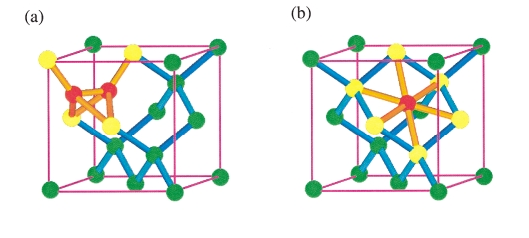
\includegraphics[width=10cm]{Figures/ab.pdf}
%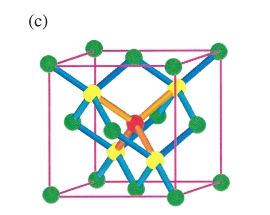
\includegraphics[width=5cm]{Figures/c.pdf}
\caption{(a) The split-110 (X) and (b) hexagonal (H) interstitial defects \cite{dow11}.}
\label{fig:Cells}
\end{center}
\begin{itemize}
	\item Defect atoms are red 
	\item Their nearest neighbors are yellow
	\item The bonds between them are orange
\end{itemize}
\end{figure}

\end{frame}

% =========================================
%==============THE CELLS=============================

\begin{frame}[plain]{The T Cell}

\begin{figure}
\begin{center}
%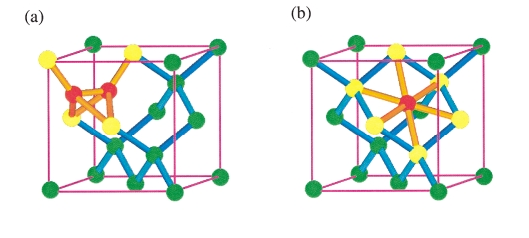
\includegraphics[width=10cm]{Figures/ab.pdf}
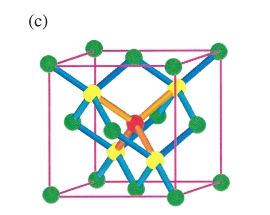
\includegraphics[width=5cm]{Figures/c.pdf}
\caption{(c) The tetrahedral (T) interstitial defect \cite{dow11}.}
\label{fig:Cells}
\end{center}
\begin{itemize}
	\item For benchmarking reasons two more interstitials are added 
	\item the vacancy (V) and the DFT-PBE hexagonal (C3V)
	\vspace{1mm}
	\begin{center}
		\textbf{All cells are relaxed using DFT-PBE}
	\end{center}
\end{itemize}
\end{figure}

\end{frame}

% =========================================
%======formation energy how to get there=============

\begin{frame}[plain]{How to calculate the Formation energy?}
	\begin{enumerate}
		\item Enegy of the Pristine cell $E_{\mathrm{bulk}}$
		\item Energy of the interstitial cell $E_{\mathrm{int}}$
	\end{enumerate}
	\vspace{5mm}
    	\begin{alertblock}{Formation Energy}
		\begin{equation*}
			E_{\mathrm{f}} = E_{\mathrm{int}} - \frac{N_{\mathrm{int}}}{N_{\mathrm{bulk}}}E_{\mathrm{bulk}}
		\end{equation*}
    	\end{alertblock}
	\vspace{5mm}
	\begin{center}
		Energies can be calculated at any level of theory
	\end{center}
\end{frame}

% =========================================
%============ccsd(t) energy how to get there=========

\begin{frame}[plain]{Workflow leading us to the converged CCSD(T) energies}
% Define block styles
\tikzstyle{block} = [rectangle, draw, fill=blue!20, text width=4em,
  text centered, rounded corners, minimum height=4em]
\tikzstyle{blockred} = [rectangle, draw, fill=red!20, text width=10em,
  text centered, rounded corners, minimum height=6em] \tikzstyle{line}
= [draw, -latex']

\begin{figure}
\begin{center}
  \begin{tikzpicture}[node distance = 2cm, auto]
  \node [blockred] (HF) {HF (VASP) \\ \noindent\rule{\linewidth}{0.4pt} \\ $\Gamma$-point};
  \node [blockred, right of=HF, node distance=5cm] (HF7) {HF increased k-point sampling (VASP) \\ \noindent\rule{\linewidth}{0.4pt} \\ 7x7x7 k-points};
  \node [blockred, below of=HF, node distance=3cm] (CC4S) {CCSD(T) (CC4S) \\ \noindent\rule{\linewidth}{0.4pt} \\ with Basis-set and Finite-size correction};
  \node [blockred, below of=HF7, node distance=3cm] (FORM) {Formation energy};

  \path [line] (HF) -- (CC4S);
  \path [line] (HF) -- (HF7);
  \path [line] (HF7) -- (FORM);
  \path [line] (CC4S) -- (FORM);
\end{tikzpicture}
	\caption{Schematic representation of the workflow}
\end{center}
\end{figure}
	
\end{frame}

% =========================================
%=============finite size error======================

\begin{frame}[plain]{Finite Size Incompleness Error}
	Due to the periodic supercell approach, we are always having a defined defect concentration
	\begin{itemize}
		\item Finite size error due to periodic images $\to$ bigger cell 
		\item Finite size error due finite number of kpoints
			\begin{itemize}
				\item In the case of HF $\to$ increase kpoints
				\item In the case of CCSD(T) $\to$ finite size correction\cite{FiniteSize}
			\end{itemize}
		\item Correction is done on one k-point $\to$ twist averaging 
			\begin{itemize}
				\item Calculate the CCSD(T) correction at random k-points
				\item Take a look at the average and standard deviation 
			\end{itemize}
	\end{itemize}
\end{frame}

% =========================================
%===========basis set error==========================

\begin{frame}[plain]{Basis Set Incompleteness Error}
	The Basis set incompleteness error comes mostly from the electron-electron cusp
	\begin{itemize}
		\item Pair-specific cusp correction in cc4s, focal-point correction (FPC)\cite{BasisSet}
	\end{itemize}
\begin{figure}[htb]
  \centering
  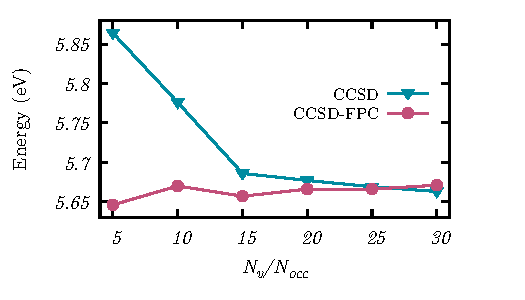
\includegraphics[width=.8\textwidth]{./Figures/BasisSetCorrection.pdf}
  \caption{%
    CCSD formation energy of the X interstitial.
    At the $\Gamma$-point}%
    \label{fig:basisSetConvergence}
\end{figure}

\end{frame}

% =========================================
%============Results=================================

\begin{frame}[plain]{Results}
\begin{table}
\centering
        \caption{Computed and converged HF, CCSD and CCSD(T) formation energies including
        all reported corrections, compared to QMC~\cite{QMCRef}, RPA~\cite{Kresse}, PBE~\cite{Kresse},
        LDA~\cite{dow7,dow10}, $G_0W_0$~\cite{dow7} and HSE~\cite{dow10} from the literature
        and also experimental data~\cite{exp2,exp4,exp5,exp6,exp7}. %All results have been obtained for the 16/17 atom cells
%        except RPA(216), which employed 216/217 atom cells.
        \label{table4}}
\resizebox{\textwidth}{!}{
\begin{tabular}{lcccccccccccc}
\toprule
Cell            &HF       &CCSD     &CCSD(T)    &QMC    &QMC (nobf)     &$G_0W_0$&RPA   &RPA (216)      &HSE    &PBE    &LDA    &Exp.           \\
\midrule
%C3V            &8.502          &5.788          &4.998          &       &               &4.51   &4.39   &4.36           &       &3.64   &3.36   &               \\
X               &7.930          &5.295          &4.535          &4.4    &4.9            &4.46   &4.27   &4.2            &4.46   &3.56   &3.29   &               \\
H               &8.162          &5.559          &4.810          &4.7    &4.9            &4.4    &4.45   &4.33           &4.82   &3.74   &3.4    &4.2 - 4.7      \\
T               &9.954          &7.127          &6.316          &5.1    &5.2            &       &4.53   &4.93           &4.92   &3.66   &3.56   &               \\
%V              &5.554          &5.070          &4.779          &       &               &       &3.47   &4.39           &       &3.02   &       &2.1 – 4.0      \\
\bottomrule
\end{tabular}}
\end{table}
	\vspace{4mm}
	\begin{itemize}
		\item X and H look good
		\item T does not look good
	\begin{itemize}
		\item Multiconfigurational character?
	\end{itemize}
	\end{itemize}
\end{frame}

% =========================================
%==================Outlook==================
\section{Outlook}
\begin{frame}[noframenumbering,plain]
    \begin{center}
    \Huge {\textcolor{faeng_blue}{Outlook}} 
    \vspace{5mm} 
    \hrule 
    \end{center}
\end{frame}
%====================================================
%====================================================

\begin{frame}[plain]{Outlook}
	\begin{itemize}
		\item Coupled Cluster is one of the most accurate Wavefunction theories in Quantum Chemistry
		\pro Can be used for systems with $\approx 50$ atoms
		\pro Ab initio - no parameters
		\pro Size extensitivity - perfect for solid state physics
		\con Only applicable to weakly correlated systems
		\con Gets expensive fast - CCSD(T) $O(N^{7})$
	\end{itemize}
\end{frame}

% =========================================
%==================thank you================
\begin{frame}[plain]{Thank you!}
    \begin{center}
	    Thank you
    \end{center}
\begin{figure}[htb]
  \centering
  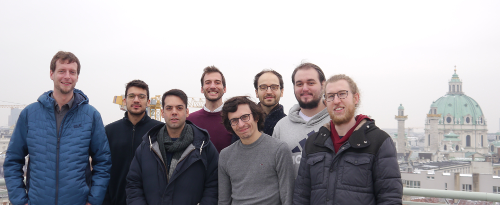
\includegraphics[width=.8\textwidth]{./Figures/group2019.png}
	\caption{Adreas Grüneis, Nikolaos Masios, Theodoros Tsatsoulis, Felix Hummel, Andreas Irmler, Alejandro Gallo, Faruk Salihbegovic, Tobias Schäfer}
\end{figure}
%\begin{figure}[htb]
%  
\includegraphics[width=.2\textwidth]{./figs/TU_Logo.pdf}
%\end{figure}
%\begin{figure}[htb]
%  
\includegraphics[width=.2\textwidth]{./figs/ERC_Logo.png}
%\end{figure}

\begin{figure}%
    \centering
    \subfloat[]{{
\includegraphics[width=3cm]{./figs/TU_Logo.pdf} }}%
    \subfloat[]{{
\includegraphics[width=2cm]{./figs/ERC_Logo.png} }}%
\end{figure}

\end{frame}
%====================================================
% =========================================

%\begin{frame}[plain]{Blocos}
%\end{frame}

% =========================================


% =========================================


% =========================================


% =========================================

\printbibliography

\end{document}

% =============================================================
% =========================== END =============================
% =============================================================

